%!TEX root = ../../report.tex
\section{Collaborative Recommendations}
\label{sec:collaborative}
The main idea of this approach for recommendations, is to base the recommendations of items on similar users or similar items.\\
This method of recommending is one of the most widely spread, as it is used both at Amazon, Netflix and similar high-value companies \todo{Kilde: Linden et al. 2003}.\\
In this section, the different implementation techniques of CF recommender systems will be described and a list of pro's and cons, be giving towards the end. We will distinguish between what is known as user-based and item-based recommendations \todo{Kilde: Recommender Systems, An Introduction}. But before going is to these descriptions, a short section for the commons features will be explained\\

For both types of recommendations the basic problem can be formulated like this: For any given user and non-rated item pair, try to estimate the rating the user will give, for this item.\\
The most common approach is therefore to define a user-item matrix as seen in the table below \todo{insert a table here}

%\subsection{Ratings} % (fold)
%\label{sub:ratings}
%A part about implicit and explicit ratings.

% subsection ratings (end)
\subsection{user-user based recommendations} % (fold)
\label{sub:user_user_based_recommendations}
The approach described here are recommending on the basis of what is known as peer-users (also called neighbors). This means users that have similar preferences in the past as the user the systems is trying to recommend items to. The idea is, for the item n, which a user called Alice not yet have rated, find peer-users that have rated item n and based on the this, compute the rating for item n for the Alice. This means that the job of the RS is to: 1) find peer-users with similar taste to Alice and 2) take the rating for the item from the peer-users and based on this, predict the rating for the item for Alice.
To illustrate this, we can return to our rating matrix in matrix \(R\). Here Alice have not rated item 4 and the task of the RS is then to predict the rating for item 4, based on the ratings of this item from peer-users, which is user2 and user4. Most commonly the is done, using the Pearson correlation coefficient\todo{KILDE?}, which calculates the similarity between users.

\subsubsection{Pearson correlation}
Before describing the mathematical formulations, we need first to establish the basic terms required for the calculations. As described in section \ref{sec:collaborative} a matrix of items and users are made. The users will in the following be denoted as \( U = {u_{1}, \ldots , u_{n}} \) , the items will be denoted as \( P = {p_{1}, \ldots , p_{n}} \) and \(R\) for the \({n x m}\) matrix for ratings \(r_{i}, r_{j}\) for \(i \in 1 \ldots n, j \in 1 \ldots m\). The possible ratings a user can give is 1-5, where 5 being the the most-liked rating option. 
The similarity between user a and user b, giving the matrix \(R\) is defined as follows:\\

\[
	sim(a,b) = \frac{\sum_{p\in P} (r_{a,p} - \bar{r_{a}})(r_{b,p} - \bar{r_{b}})}{\sqrt{\sum_{p\in P} (r_{a,p} - \bar{r_{a}})^2} \sqrt{\sum_{p\in P} (r_{b,p} - \bar{r_{b}})^2}}
\]


This will produce the similarity of user a and user b to be \todo{XXX}. This is a relatively high similarity and using the same formula for user a and user c, we also end up with a high similarity. It should be noted, that the formula takes into account that users tends to interpret a rating scale differently. Meaning that, some users tend to give a lot of high ratings, whereas other never rates anything with a 5. 
Now that we have found two users (b and c), that have rated items similar to user a, we are able to proceed and predict rating for the items, user a not yet have rated. According to \todo{kilde til RS, an Introduction, p16} one possible way of making the prediction is based on this formula:\\

\[
	pred(a,p) = \bar{r_{a}} + \frac{\sum_{b\in N} sim(a,b) * (r_{b,p} - \bar{r_{b}})}{\sum_{b\in N} sim(a,b)}
\]

Based on these predictions, we are now able to fill out the rating matrix for user a and making a list of top recommendations, based on this matrix. \\

The above presentation of a recommender systems is of course a very small example and in real world applications, the case of recommending is not a straight-forward as the method described here. The example just holds 4 users and 5 items, whereas real-world applications often contains tens of thousand or even millions of both items and users, which was the case for the Netflix problem\todo{kilde netflix problem}. As we will later present, a problem about data sparsity with rating for items, is also a very present and problematic issue for recommendations systems. \todo{Problems with scalability} 

% subsection user_user_based_recommendations (end) 

\subsection{item based recommendations} % (fold)
\label{sub:item_based_recommendations}
Another technique of collaborative recommendations, called item-based, are in certain areas very similiar to user-based technique described above, but has some advantages in the sense of the large dataset an real-world application consists of today. The main idea of this approach is to calculate the similarity between items, instead of users, based on ratings for the items. If we want to compute the rating for item5 and we return to our matrix\todo{MATRIX}, we can see that the ratings given for item5, is close to the ratings given for both item2 and item4. Because of this similarity, we can say that: Since user a gave a rating of 4 to item2 and user b gave a rating of 3 to item4, item2 and item4 is similar in theirs ratings, a item-based recommender system will compute the average of these similar items ratings and give item5 a rating between 3 and 4. \todo{Bedre eksempel. p19}
In the following a description of one item-based algorithm will be presented. 

\subsubsection{Cosine similarity measure}
In the previous sections, we looked at how item5 had similar ratings as item2 and item4.Because of a small dataset, it was possible to observe this similarity without any kind of calculations. It is rarely the case that this is possible in real-world applications and one of the methods for calculating this similarity is to use the cosine similarity measure. Making a vector from each of the items, based on their ratings, this method uses the angle between the two vector for measuring of their similarity. The formula for calculating this angle is found below:

\[
	sim(\vec{a}, \vec{b}) = \frac{\vec{a} \cdot \vec{b}}{|\vec{a}| * |\vec{b}| }
\]

\todo{explanation of the formula}

The cosine similarity values goes from -1, trough 0 and to 1, where 1 indicates a strong similarity between the two compared items, just like the Pearson method, as indicated on the picture below:

\begin{figure}[ht!]
\centering
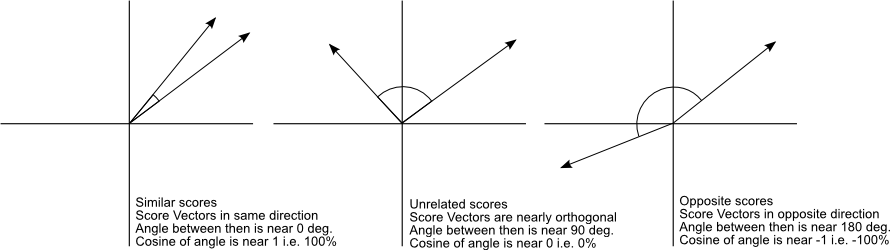
\includegraphics[width=90mm]{Pictures/cosinesimilarity.png}
\caption{source: http://pyevolve.sourceforge.net/wordpress/?p=2497}
\label{cosinesimilarity}
\end{figure}

Differently from the Pearson method, the formula does not take into account that users use a rating scale differently. \todo{maybe note the adjusted cosine measure her? p19}
After the similarity between the items have been calculated, the recommender system can predict a rating for user a's item5, based on the ratings for the items similar to item5. This prediction is done, using the formula below:

\[
	pred(u,p) = \frac{\sum_{i\in ratedItems(u)} sim(i,p) * r_{u,i}}{\sum_{i \in ratedItems(a)} sim(i,p)}
\]

\subsubsection{Data sparsity and cold start problem}
\label{subsec:data_sparsity}
% subsection user_item_based_recommendations (end)
\todo{section: Data preprocessing}

\subsection{Advantages and disadvantages}
According to \todo{kilde: Recommender systems, an introduction} collaborative recommender systems is one of the most researched techniques of the two and because of this many different types of collaborative recommendations exists, as described in the above. Even with many different types, it is possible to outline some common advantages and disadvantages, which we be done in this section. Firstly, collaborative filtering can work independent of the items the system holds, since it uses ratings to recommender from, as opposed to content-based, which requires the item to have some content that can be compared \todo{kilde The next generation of recommender system, p18(nederst)}. 
\todo{more advantages?}
Likewise with content-based recommender method, the collaborative method do also have some disadvantages, or more correct, some challenges, described here as: New user problem, new item problem and data sparsity. 
\begin{itemize}
	\item New users are both problem for both methods, since both relies on some previous history about the users. In order for a recommender system to make recommendations for a user, the system must know something about the user preferences, which is historic ratings in a collaborative system. 
	\item New items are frequently being added to a systems 'inventory'. This creates a challenge for a collaborative based recommender system, since it relies upon ratings for the items it recommends, and which it obviously does not have for new items.  
\end{itemize}